% CS.tex

\chapter{Grille Cubed-Sphère}

\section{Définition géométrique de la Cubed-Sphère}

\subsection{La sphère $\mathbb{S}_a^2$}

Soit $a > 0$ un réel strictement positif. $\mathbb{S}_a^2$ est la sphère de centre $O : (0,0,0) \in \mathbb{R}^3$ et de rayon $a$ :

\begin{equation}
\mathbb{S}_a^2 := \left\lbrace
\mathbf{x} = (x,y,z)^T \in \mathbb{R}^3 \text{ tels que } x^2+y^2+z^2 = a^2
\right\rbrace
\end{equation} 

On nomme grand cercle, un cercle de centre $O$ et de rayon $a$. Un grand cercle est inclus dans la sphère $\mathbb{S}_a^2$.
Soient $C_1$ et $C_2$ deux grands cercles distincts, $\mathbf{x} \in C_1 \cap C_2$ alors $\mathbf{x} \in \mathbb{S}_a^2$.
On pose les points $\mathbf{x}_1 \in C_1$ et $\mathbf{x}_2 \in C_2$, on peut alors définir $\alpha$ (resp. $\beta$) l’abscisse curviligne de $\mathbf{x}$ le long de $C_1$ (resp. $C_2$) avec $\mathbf{x}_1$ (resp. $\mathbf{x}_2$) comme origine (Voir figure \ref{fig: grands cercles}).


\begin{figure}[ht]
\begin{center}
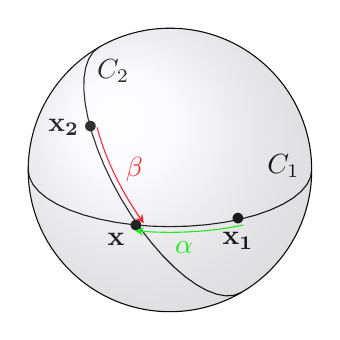
\begin{tikzpicture}[scale=1.8]
	% \draw [color=gray] (-1.5,-1.5) grid[step=0.1] (1.5,1.5);
	\draw [domain=0:-180] plot({cos(\x)},{0.4*sin(\x)});
	\draw (0.8,0.03) node {$C_1$} ;  
	\draw [rotate=-60,domain=0:-180] plot({cos(\x)},{0.4*sin(\x)});
	\draw (-0.4,0.7) node {$C_2$} ; 
	\draw (-0.24,-0.4) node {$\bullet$} ;
	\draw (-0.38,-0.49) node {$\mathbf{x}$} ;
	\draw (0.48,-0.35) node {$\bullet$} ;
	\draw (0.48,-0.5) node {$\mathbf{x_1}$} ;
	\draw [>=stealth, ->,color=green,domain=-62:-103] plot({1.1*cos(\x)},{0.44*sin(\x)});
	\draw [color=green] (0.1,-0.55) node {$\alpha$} ;
	\draw (-0.56,0.3) node {$\bullet$} ;
	\draw (-0.75,0.3) node {$\mathbf{x_2}$} ;
	\draw [rotate=-60,>=stealth, <-,color=red,domain=-75:-125] plot({0.9*cos(\x)},{0.36*sin(\x)});
	\draw [color=red] (-0.25,0) node {$\beta$} ;
    \draw (0,0) circle (1cm);
    \shade[ball color=blue!10!white,opacity=0.20] (0,0) circle (1cm);
\end{tikzpicture}
\end{center}
\caption{Grandes cercles sur la sphère $\mathbb{S}_a^2$.}
\label{fig: grands cercles}
\end{figure}

En tout point $\mathbf{x} \in \mathbb{S}_a^2$, il existe un plan tangent à la sphère noté $\mathbb{T}_{\mathbf{x}}\mathbb{S}_a^2$. Il est engendré par les vecteurs $\mathbf{e}_{\alpha}$ et $\mathbf{e}_{\beta}$ (Voir figure \ref{fig: e_alpha et e_beta}) donnés par :

\begin{equation}
\mathbf{e}_{\alpha} := \dfrac{\partial \mathbf{x}}{\partial \alpha} \text{ et } \mathbf{e}_{\beta} := \dfrac{\partial \mathbf{x}}{\partial \beta}
\end{equation}

\begin{figure}[ht]
\begin{center}
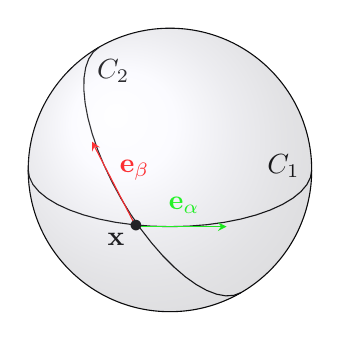
\begin{tikzpicture}[scale=1.8]
	\draw [domain=0:-180] plot({cos(\x)},{0.4*sin(\x)});
	\draw (0.8,0.03) node {$C_1$} ;  
	\draw [rotate=-60,domain=0:-180] plot({cos(\x)},{0.4*sin(\x)});
	\draw (-0.4,0.7) node {$C_2$} ; 
	
	\draw [>=stealth, ->, color=green] (-0.24,-0.4) -- (0.4,-0.4) ;
	\draw [color=green] (0.1,-0.25) node {$\mathbf{e}_{\alpha}$} ;	
	\draw [>=stealth, ->, color=red] (-0.24,-0.4) -- (-0.55,0.2) ;	
	\draw [color=red] (-0.25,0) node {$\mathbf{e}_{\beta}$} ;
	
	\draw (-0.24,-0.4) node {$\bullet$} ;
	\draw (-0.38,-0.49) node {$\mathbf{x}$} ;
	\draw (0,0) circle (1cm);
    \shade[ball color=blue!10!white,opacity=0.20] (0,0) circle (1cm);
\end{tikzpicture}
\end{center}
\caption{Grandes cercles sur la sphère $\mathbb{S}_a^2$.}
\label{fig: e_alpha et e_beta}
\end{figure}

A partir de ces vecteurs $\mathbf{e}_{\alpha}$ et $\mathbf{e}_{\beta}$, une base duale de $\mathbb{T}_{\mathbf{x}}\mathbb{S}_a^2$, notée $\left( \mathbf{e}^{\alpha}, \mathbf{e}^{\beta} \right)$, est donnée grâce aux relations suivantes :

\begin{equation}
\left\lbrace
\begin{array}{rcccl}
\mathbf{e}_{\alpha} \cdot \mathbf{e}^{\alpha} & = & 1 & = & \mathbf{e}_{\beta} \cdot \mathbf{e}^{\beta} \\
\mathbf{e}_{\alpha} \cdot \mathbf{e}^{\beta} & = & 0 & = & \mathbf{e}_{\beta} \cdot \mathbf{e}^{\alpha} \\
\end{array}
\right.
\label{eq: dualite alpha beta}
\end{equation}

Il est important de noter que les vecteurs $\mathbf{e}_{\alpha}$, $\mathbf{e}_{\beta}$, $\mathbf{e}^{\alpha}$ et $\mathbf{e}^{\beta}$ dépendent de la position du point $\mathbf{x}$. 
Si $h : \mathbf{S}_a^2 \mapsto \mathbb{R}$ est une fonction régulière sur la sphère, son gradient est donné par :

\begin{equation}
\nabla_{T} h := \dfrac{\partial h}{\partial \alpha} \mathbf{e}_{\alpha} + \dfrac{\partial h}{\partial \beta} \mathbf{e}_{\beta}
\label{eq: gradient}
\end{equation}

\begin{proposition}
Le gradient \eqref{eq: gradient} est bien définit. Il ne dépend pas du choix des deux grands cercles $C_1$ et $C_2$ choisis.
\end{proposition}

\begin{proof}
Soient $\tilde{C}_1$ et $\tilde{C}_2$ deux grands cercles distincts entre eux et distincts de $C_1$ et $C_2$. $\tilde{\alpha}$ et $\tilde{\beta}$ les abscisses curvilignes associées. On pose :
\begin{equation}
\mathbf{e}_{\tilde{\alpha}} = \dfrac{\partial \mathbf{x}}{\partial \tilde{\alpha}} \text{ et } \mathbf{e}_{\tilde{\beta}} = \dfrac{\partial \mathbf{x}}{\partial \tilde{\beta}}
\end{equation}

la base de $\mathbb{T}\mathbb{S}_a^2$ associée à $(\tilde{\alpha}$ et $\tilde{\beta}$. $\left( \mathbf{e}^{\tilde{\alpha}}, \mathbf{e}^{\tilde{\beta}} \right)$ est construite par dualité :

\begin{equation}
\left\lbrace
\begin{array}{rcccl}
\mathbf{e}_{\tilde{\alpha}} \cdot \mathbf{e}^{\tilde{\alpha}} & = & 1 & = & \mathbf{e}_{\tilde{\beta}} \cdot \mathbf{e}^{\tilde{\beta}} \\
\mathbf{e}_{\tilde{\alpha}} \cdot \mathbf{e}^{\tilde{\beta}} & = & 0 & = & \mathbf{e}_{\tilde{\beta}} \cdot \mathbf{e}^{\tilde{\alpha}} \\
\end{array}
\right.
\end{equation}

Le problème est de savoir si $\dfrac{\partial h}{\partial \alpha} \mathbf{e}^{\alpha} + \dfrac{\partial h}{\partial \beta} \mathbf{e}^{\beta}$ est égal à $\dfrac{\partial h}{\partial \tilde{\alpha}} \mathbf{e}^{\tilde{\alpha}} + \dfrac{\partial h}{\partial \tilde{\beta}} \mathbf{e}^{\tilde{\beta}}$.

D'un part, on a :

\begin{equation}
\begin{array}{rcl}
\mathbf{e}_{\alpha} & = & \dfrac{\partial \tilde{\alpha}}{\partial \alpha} \mathbf{e}^{\tilde{\alpha}} + \dfrac{\partial \tilde{\beta}}{\partial \alpha} \mathbf{e}^{\tilde{\beta}} \\
\mathbf{e}_{\beta} & = & \dfrac{\partial \tilde{\alpha}}{\partial \beta} \mathbf{e}^{\tilde{\alpha}} + \dfrac{\partial \tilde{\beta}}{\partial \beta} \mathbf{e}^{\tilde{\beta}} \\
\end{array}
\end{equation}

De plus :

\begin{equation}
\dfrac{\partial h}{\partial \tilde{\alpha}} \mathbf{e}^{\tilde{\alpha}} + \dfrac{\partial h}{\partial \tilde{\beta}} \mathbf{e}^{\tilde{\beta}} = \dfrac{\partial h}{\partial \alpha}  \underbrace{\left( \dfrac{\partial \alpha}{\partial \tilde{\alpha}} \mathbf{e}^{\tilde{\alpha}} + \dfrac{\partial \alpha}{\partial \tilde{\beta}} \mathbf{e}^{\tilde{\beta}}  \right)} _{=\mathbf{u}} + \dfrac{\partial h}{\partial \alpha}  \underbrace{\left( \dfrac{\partial \beta}{\partial \tilde{\alpha}} \mathbf{e}^{\tilde{\alpha}} + \dfrac{\partial \beta}{\partial \tilde{\beta}} \mathbf{e}^{\tilde{\beta}} \right)}_{= \mathbf{v}} 
\label{eq: prop u v}
\end{equation}

On cherche à savoir quel est le lien entre $\mathbf{u}$, $\mathbf{v}$ avec $\mathbf{e}^{\alpha}$ et $\mathbf{e}^{\beta}$.

\begin{equation}
\mathbf{e}_{\alpha} \cdot \mathbf{u} = \dfrac{\partial \tilde{\alpha}}{\partial \alpha} \dfrac{\partial \alpha}{\partial \tilde{\alpha}} + \dfrac{\partial \tilde{\beta}}{\partial \alpha} \dfrac{\partial \alpha}{\partial \tilde{\beta}} = \dfrac{\partial \alpha}{\partial \alpha} = 1.
\end{equation}

De même : $\mathbf{e}_{\beta} \cdot \mathbf{v} = 1$.

De la même manière, on a :

\begin{equation}
\mathbf{e}_{\alpha} \cdot \mathbf{v} = \dfrac{\partial \tilde{\alpha}}{\partial \alpha} \dfrac{\partial \beta}{\partial \tilde{\alpha}} + \dfrac{\partial \tilde{\beta}}{\partial \alpha} \dfrac{\partial \beta}{\partial \tilde{\beta}} = \dfrac{\partial \beta}{\partial \alpha} = 0.
\end{equation}

Ainsi que $\mathbf{e}_{\beta} \cdot \mathbf{u} = 0$.

Donc $\mathbf{u}$ et $\mathbf{v}$ vérifient \eqref{eq: dualite alpha beta}. De plus, $\mathbf{u}, \mathbf{v} \in \mathbb{T}_{\mathbf{x}} \mathbb{S}_a^2$. Donc $\mathbf{u} = \mathbf{e}^{\alpha}$ et $\mathbf{v} = \mathbf{e}^{\beta}$. Ainsi, en utilisant \eqref{eq: prop u v}, on a bien :

\begin{equation}
\dfrac{\partial h}{\partial \tilde{\alpha}} \mathbf{e}^{\tilde{\alpha}} + \dfrac{\partial h}{\partial \tilde{\beta}} \mathbf{e}^{\tilde{\beta}} = \dfrac{\partial h}{\partial \alpha} \mathbf{e}^{\alpha} + \dfrac{\partial h}{\partial \beta} \mathbf{e}^{\beta}
\end{equation}

Le gradient est bien définit car indépendant du choix des grands cercles.
\end{proof}

\begin{proposition}
Soit $\mathbf{x} \in \mathbb{S}_a^2$, alors $\nabla_{T} h (\mathbf{x}) \in \mathbb{T}_{\mathbf{x}} \mathbb{S}_a^2$.
\end{proposition}

\begin{proof}
$\nabla_{T} h (\mathbf{x})$ est une combinaison linéaire de $\mathbf{e}^{\alpha}(\mathbf{x})$ et $\mathbf{e}^{\beta}(\mathbf{x})$. Ces deux vecteurs engendrent le plan $\mathbb{T}_{\mathbf{x}}\mathbb{S}_a^2$, d'où le résultat.
\end{proof}

\begin{proposition}
Soit $u: \mathbb{R}^3 \mapsto \mathbb{R}$ une fonction de $\mathbb{R}^3$ et $\mathbf{x} \in \mathbb{R}^3$. On pose $\hat{u} : = u_{|\mathbb{S}_a^2}$ la restriction de $u$ à la sphère $\mathbb{S}_a^2$. Alors $\nabla_{T} \hat{u} (\mathbf{x})$ est la projection orthogonale de $\nabla_{\mathbb{R}^3} u (\mathbf{x})$ sur le plan tangent $\mathbb{T}_{\mathbf{x}} \mathbb{S}_a^2$.

\begin{equation}
\nabla_T \hat{u} = \nabla_{\mathbb{R}^3} u - \mathbf{n} \left( \mathbf{n} \cdot \nabla_{\mathbb{R}^3} u \right)
\end{equation}

avec $\mathbf{n}$ la normale unitaire extérieure.
\end{proposition}

\begin{proof}
TBA
\end{proof}





\subsection{Construction de la Cubed-Sphère}













\section{Coordonnées Gnomoniques}


















\section{Calcul intrinsèque sur la Cubed-Sphère}


















